% Created 2015-04-08 Wed 22:37
\documentclass[11pt]{article}
\usepackage[utf8]{inputenc}
\usepackage[T1]{fontenc}
\usepackage{fixltx2e}
\usepackage{graphicx}
\usepackage{longtable}
\usepackage{float}
\usepackage{wrapfig}
\usepackage{rotating}
\usepackage[normalem]{ulem}
\usepackage{amsmath}
\usepackage{textcomp}
\usepackage{marvosym}
\usepackage{wasysym}
\usepackage{amssymb}
\usepackage{hyperref}
\tolerance=1000
\usepackage[margin=1in]{geometry}
\author{Constantine Khroulev}
\date{\today}
\title{Modeling orographic precipitation}
\hypersetup{
  pdfkeywords={},
  pdfsubject={},
  pdfcreator={Emacs 24.4.90.1 (Org mode 8.2.10)}}
\begin{document}

\maketitle
\tableofcontents


\section{Intro}
\label{sec-1}

Simple upslope precipitation models such as the one used in
\cite{roe2003orographic} and \cite{roe1999wobbly} are \textbf{local}
functions of wind speed, surface slope, and (through a temperature
parameterization) surface elevation.

This implies that
\begin{itemize}
\item Locations with similar slopes and elevations will get similar
amounts of even if one of them is located farther from the
moisture source.
\item It is difficult to create a setup in which surface topography
affects the distribution of precipitation, but not its \textbf{total}
over the modeling domain.
\end{itemize}

We can use a moisture transport model due to
\cite{sanberg1983modelling}, which is similar to
\cite{roe2003orographic} in the way it parameterizes precipitation:

\begin{equation}
\frac{\partial W}{\partial t} = -\vec v \cdot \nabla W - (f_0 + f_1 S) W + (W_m - W) / T_{*} + D_w \nabla^2 W
\end{equation}

Sanberg and Oerlemans implement this using a finite difference
approximation and explicit time stepping and iterate until a steady
state is reached. In \cite{sanberg1983modelling} the precipitation
pattern is updated once every 500 years of ice sheet evolution.

This model was successfully used by \cite{letreguilly1993modelling}
to model the Fennoscandian ice sheet.

\subsection{Steady-state flow-line setup}
\label{sec-1-1}

In a steady-state flow-line case we can model the moisture source
by prescribing Dirichlet boundary conditions over the ocean.

Note also that $\partial W / \partial x = - p(x)$, so omitting the
diffusion term results in the form equivalent to equation (4.19) in
\cite{roe1999wobbly}:
\begin{equation}
P = (\gamma'_0 + \gamma'_1 S) W.
\end{equation}

In turn, assuming that $W$ is proportional to $e_s(T)$ gives
\begin{equation}
P = \left( \alpha_0 + \alpha_1 \cdot v \cdot \frac{\partial z}{\partial x} \right) e_s(T),
\end{equation}
which is equation (9) in \cite{roe2003orographic} interpreted as precipitation.

\subsection{Flow-line implementation details}
\label{sec-1-2}

Equation (4.16) in \cite{roe1999wobbly} includes an important
detail: one has to make sure that a parameterization produces
non-negative precipitation values.

We solve
\begin{align}
  \frac{\partial W}{\partial x} &= -W \max\left(\alpha_0 + \alpha_1 \cdot v \cdot \frac{\partial z}{\partial x}, 0 \right),\\
  W(0) &= 1.
\end{align}

to determine the distribution of precipitation. This model \textbf{reduces}
precipitation on the lee side of a mountain, because as cold
saturated air travels downhill it gets warmer and less saturated.

Roe \cite{roe1999wobbly} also mentions that
\cite{sanberg1983modelling} set $S$ to zero in areas where air is
traveling downhill.

To use this variation of the model, we solve
\begin{align}
  \frac{\partial W}{\partial x} &= -W \left( \alpha_0 + \max\left(\alpha_1 \cdot v \cdot \frac{\partial z}{\partial x}, 0 \right) \right),\\
  W(0) &= 1.
\end{align}

Note: we may need to add a diffusion term to get an effect similar
to "upwind smoothing" of \cite{roe2003orographic}.

\section{Implementation prototype}
\label{sec-2}
\begin{verbatim}
#!/usr/bin/env python

from scipy.integrate import odeint
import numpy as np
import pylab as plt

def bump(x, x0, d_minus, d_plus):
    """a smooth 'bump' centered at x0, with 'characteristic distances'
    d_minus and d_plus for parts x <= x0 and x > x0 respectively

    We create this by matching two Gaussian bumps that are scaled
    using d_minus and d_plus.

    """
    def _bump(x):
        if x <= x0:
            d = d_minus
        else:
            d = d_plus
        return np.exp(-(x - x0)**2 / (2.0 * d**2))

    return np.vectorize(_bump)(x)

def z(x, z_max):
    "Top surface elevation as a function of x and the max. height."
    return z_max * bump(x, 5.0, 1.0, 1.0) + 0.5 * z_max * bump(x, 9.0, 1.0, 1.0)

def W_reduce_on_lee_side(W, x, alpha0, alpha1, z_max):
    """Right hand side of dM/dx = C * M. Note that dM/dx = -p(x).

    This parameterization reduces precipitation on the lee side. (Cold
    saturated air traveling down a mountain warms up and becomes less
    saturated.)

    """
    dx = 0.01
    dz = z(x + dx, z_max) - z(x, z_max)
    return -W * max(alpha0 + alpha1 * v * dz / dx, 0.0)

def W_dont_reduce_on_lee_side(W, x, alpha0, alpha1, z_max):
    """Right hand side of dM/dx = C * M. Note that dM/dx = -p(x).

    This parameterization does not include the influence of the wind
    speed and the surface slope on the lee side. (This is equivalent
    to setting alpha1 to zero in the lee side.)

    """
    dx = 0.01
    dz = z(x + dx, z_max) - z(x, z_max)
    return -W * (alpha0 + max(alpha1 * v * dz / dx, 0.0))

# Wind speed. Changing it by a factor K is equivalent to changing
# alpha1 by the same factor, so we hold v fixed.
v = 1.0

# Initial moisture content. Should always be 1.0 because this can be
# interpreted as 100%, which is nice.
W_ocean = 1.0

x = np.linspace(0, 16, 201)

def compute(p, alpha0, alpha1, z_max):
    """Compute the distribution of the moisture content and its derivative
    (the precipitation rate).

    """
    W = odeint(p, W_ocean, x, args=(alpha0, alpha1, z_max))
    precipitation = - np.diff(W[:,0]) / (x[1] - x[0])
    return W[:,0], precipitation

def plot(p, alpha0, alpha1, z_max, title, color):
    """Plot moisture content and precipitation for a given
    parameterization and parameter choices.

    """
    W, dW = compute(p, alpha0, alpha1, z_max)
    plt.hold(True)
    plt.grid(True)
    plt.plot(x, W, "--", color=color, label="W (%s)" % title)
    plt.plot(x[1:], dW, "-", lw=2, color=color, label="precip. (%s)" % title)
    plt.legend(loc='upper right', fontsize=10)
    plt.xticks(np.linspace(0, 16, 17), [])
    plt.yticks([0])
    plt.title("max(z) = %3.3f" % z_max)
    plt.axis(ymax=W_ocean, ymin=-0.1)

alpha0 = 0.1
alpha1 = 0.1

def plot_precipitation(p, z_max):
    """For a given parameterization and mountain height, plot graphs
    exploring the effect of the background precipitation term and the
    term modeling upward motion of the air mass.

    """
    y_scale = W_ocean / z_max
    y = y_scale * z(x, z_max)
    plt.plot(x, y, color="black", label="$z$ (scaled surface elevation)")
    plot(p, alpha0, 0.0, z_max, r"$\alpha_1$ = 0", "red")
    plot(p, 0.0, alpha1, z_max, r"$\alpha_0$ = 0", "blue")
    plot(p, alpha0, alpha1, z_max,
         "$\\alpha_0$ = %3.3f, $\\alpha_1$ = %3.3f" % (alpha0, alpha1),
         "green")

def plot_parameterization(p, n1, n2):
    "Plot mountain height dependence for a given parameterization."
    plt.subplot(2, 2, n1)
    plot_precipitation(p, 2.0)
    plt.subplot(2, 2, n2)
    plot_precipitation(p, 20.0)

f = plt.figure(figsize=(20,10))
f.text(0.35, 0.975, "decrease p on the lee side",
       horizontalalignment="right",
       verticalalignment="top")
f.text(0.65, 0.975, "don't decrease p on the lee side",
       horizontalalignment="left",
       verticalalignment="top")
plot_parameterization(W_reduce_on_lee_side, 1, 3)
plot_parameterization(W_dont_reduce_on_lee_side, 2, 4)

output_filename = "orographic-precip.png"
plt.savefig(output_filename)
return output_filename          # you'll need to remove this to run it as a script
\end{verbatim}

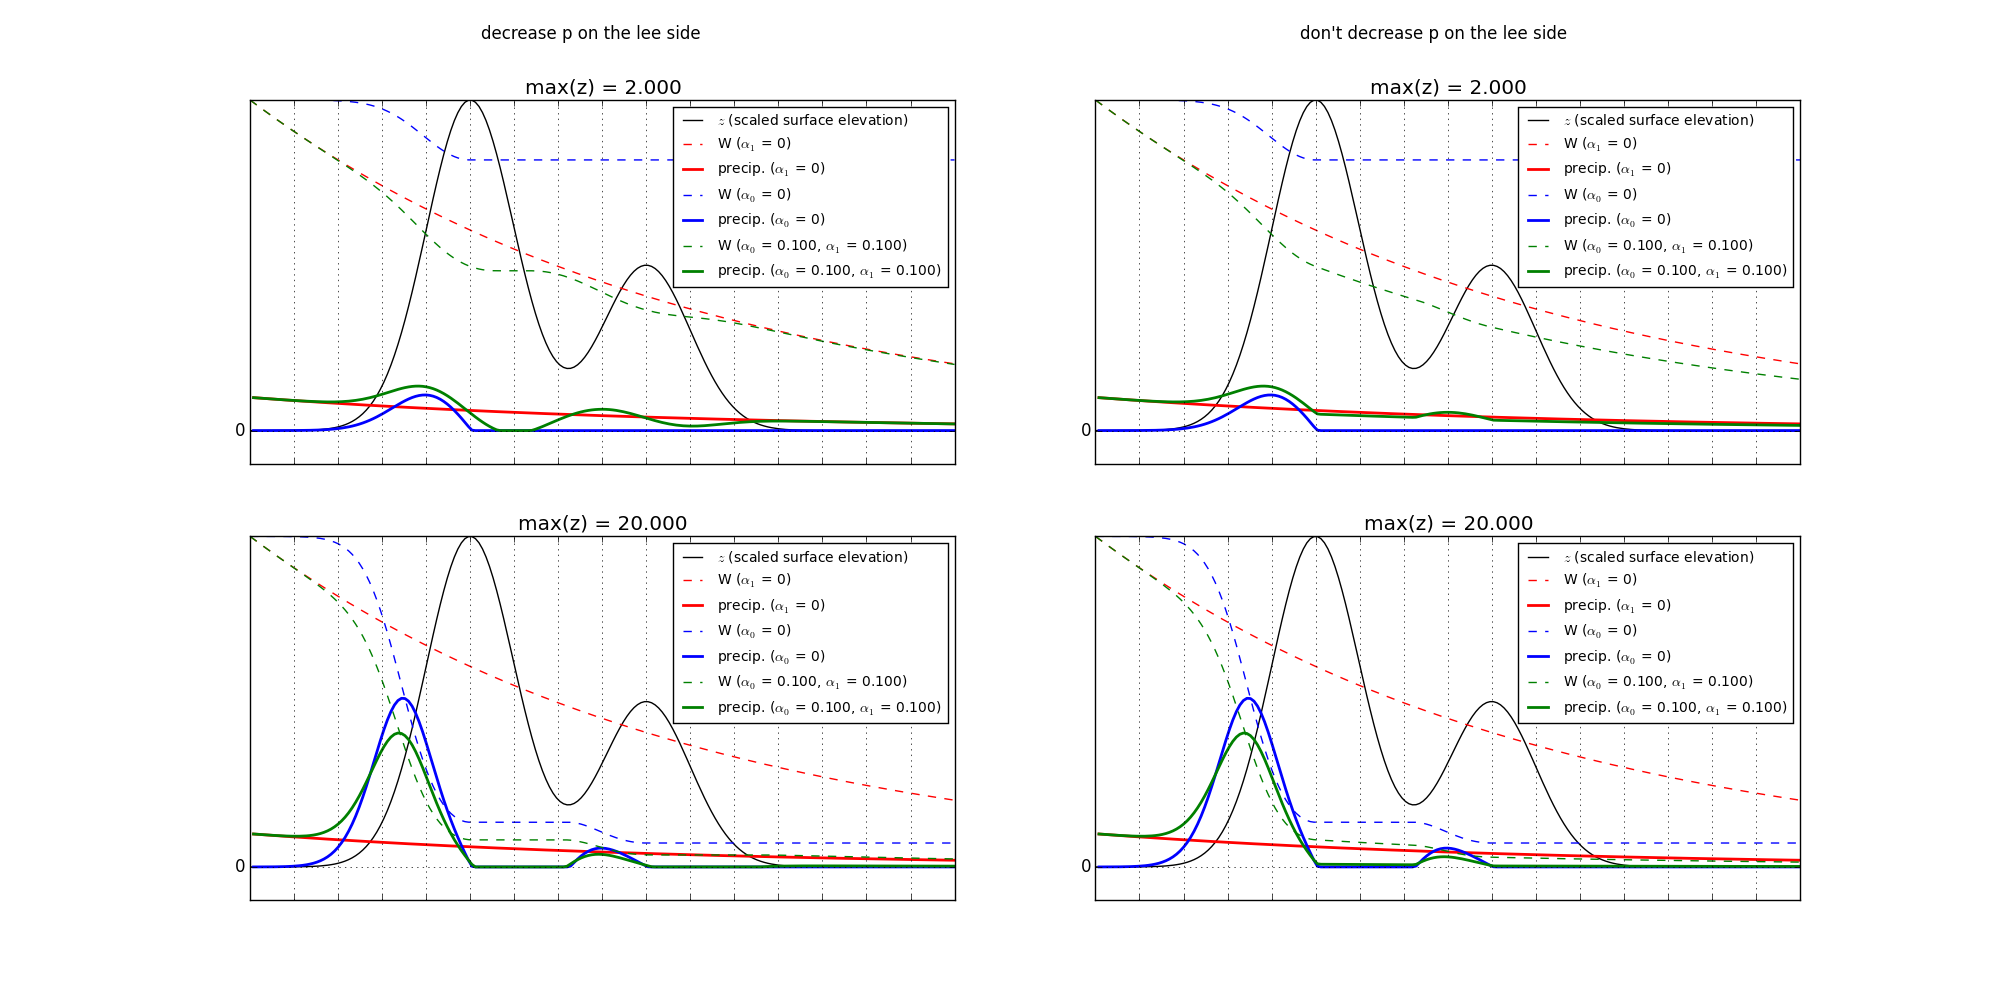
\includegraphics[width=.9\linewidth]{orographic-precip.png}

\bibliography{references}
\bibliographystyle{plain}
% Emacs 24.4.90.1 (Org mode 8.2.10)
\end{document}